% Options for packages loaded elsewhere
\PassOptionsToPackage{unicode}{hyperref}
\PassOptionsToPackage{hyphens}{url}
%
\documentclass[
]{article}
\usepackage{lmodern}
\usepackage{amssymb,amsmath}
\usepackage{ifxetex,ifluatex}
\ifnum 0\ifxetex 1\fi\ifluatex 1\fi=0 % if pdftex
  \usepackage[T1]{fontenc}
  \usepackage[utf8]{inputenc}
  \usepackage{textcomp} % provide euro and other symbols
\else % if luatex or xetex
  \usepackage{unicode-math}
  \defaultfontfeatures{Scale=MatchLowercase}
  \defaultfontfeatures[\rmfamily]{Ligatures=TeX,Scale=1}
\fi
% Use upquote if available, for straight quotes in verbatim environments
\IfFileExists{upquote.sty}{\usepackage{upquote}}{}
\IfFileExists{microtype.sty}{% use microtype if available
  \usepackage[]{microtype}
  \UseMicrotypeSet[protrusion]{basicmath} % disable protrusion for tt fonts
}{}
\makeatletter
\@ifundefined{KOMAClassName}{% if non-KOMA class
  \IfFileExists{parskip.sty}{%
    \usepackage{parskip}
  }{% else
    \setlength{\parindent}{0pt}
    \setlength{\parskip}{6pt plus 2pt minus 1pt}}
}{% if KOMA class
  \KOMAoptions{parskip=half}}
\makeatother
\usepackage{xcolor}
\IfFileExists{xurl.sty}{\usepackage{xurl}}{} % add URL line breaks if available
\IfFileExists{bookmark.sty}{\usepackage{bookmark}}{\usepackage{hyperref}}
\hypersetup{
  pdftitle={information plot},
  pdfauthor={Joshua},
  hidelinks,
  pdfcreator={LaTeX via pandoc}}
\urlstyle{same} % disable monospaced font for URLs
\usepackage[margin=1in]{geometry}
\usepackage{graphicx,grffile}
\makeatletter
\def\maxwidth{\ifdim\Gin@nat@width>\linewidth\linewidth\else\Gin@nat@width\fi}
\def\maxheight{\ifdim\Gin@nat@height>\textheight\textheight\else\Gin@nat@height\fi}
\makeatother
% Scale images if necessary, so that they will not overflow the page
% margins by default, and it is still possible to overwrite the defaults
% using explicit options in \includegraphics[width, height, ...]{}
\setkeys{Gin}{width=\maxwidth,height=\maxheight,keepaspectratio}
% Set default figure placement to htbp
\makeatletter
\def\fps@figure{htbp}
\makeatother
\setlength{\emergencystretch}{3em} % prevent overfull lines
\providecommand{\tightlist}{%
  \setlength{\itemsep}{0pt}\setlength{\parskip}{0pt}}
\setcounter{secnumdepth}{-\maxdimen} % remove section numbering

\title{information plot}
\author{Joshua}
\date{25/05/2020}

\begin{document}
\maketitle

\begin{verbatim}
##             DGP         DJ         CF
## 40   0.05110683 0.06146656 0.06273143
## 120  0.05183022 0.06108898 0.06187495
## 480  0.05108724 0.05982858 0.06036624
## 1200 0.05165158 0.06023512 0.06062999
## 4800 0.05182204 0.06011936 0.06062203
\end{verbatim}

\begin{verbatim}
##             DGP         DJ         CF
## 40   0.05153875 0.06889684 0.07089260
## 120  0.05227944 0.06554175 0.06717935
## 480  0.05126524 0.06340225 0.06507117
## 1200 0.05237592 0.06422743 0.06576759
## 4800 0.05384509 0.06545530 0.06716274
\end{verbatim}

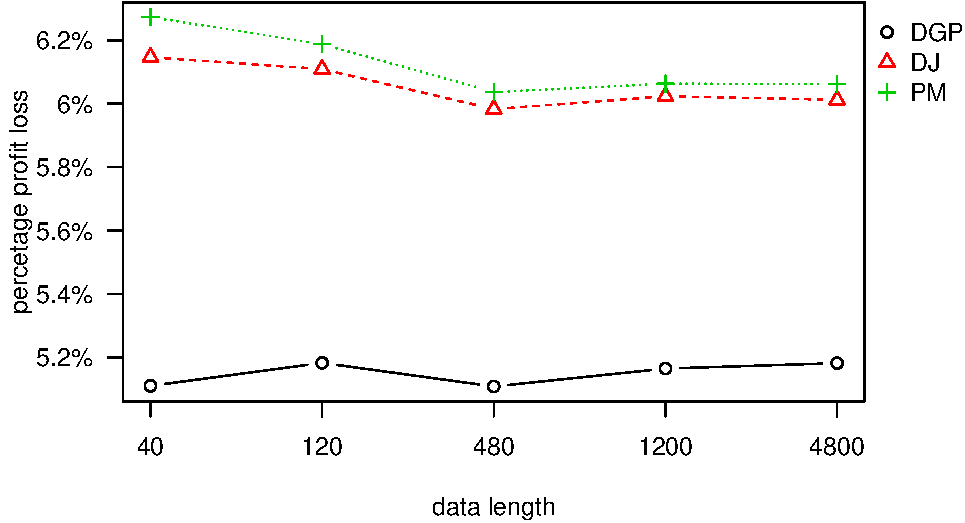
\includegraphics{information-plot_files/figure-latex/AR(1)-1.pdf}

\begin{verbatim}
##             DGP         DJ         CF
## 40   0.05110683 0.05752769 0.06098831
## 120  0.05183022 0.05378941 0.05558265
## 480  0.05108724 0.05127907 0.05253498
## 1200 0.05165158 0.05163868 0.05278057
## 4800 0.05182204 0.05179832 0.05268288
\end{verbatim}

\begin{verbatim}
##             DGP         DJ         CF
## 40   0.05153875 0.05468352 0.06648742
## 120  0.05227944 0.05167709 0.05832539
## 480  0.05126524 0.05010419 0.05398387
## 1200 0.05237592 0.05161101 0.05470931
## 4800 0.05384509 0.05366830 0.05577284
\end{verbatim}

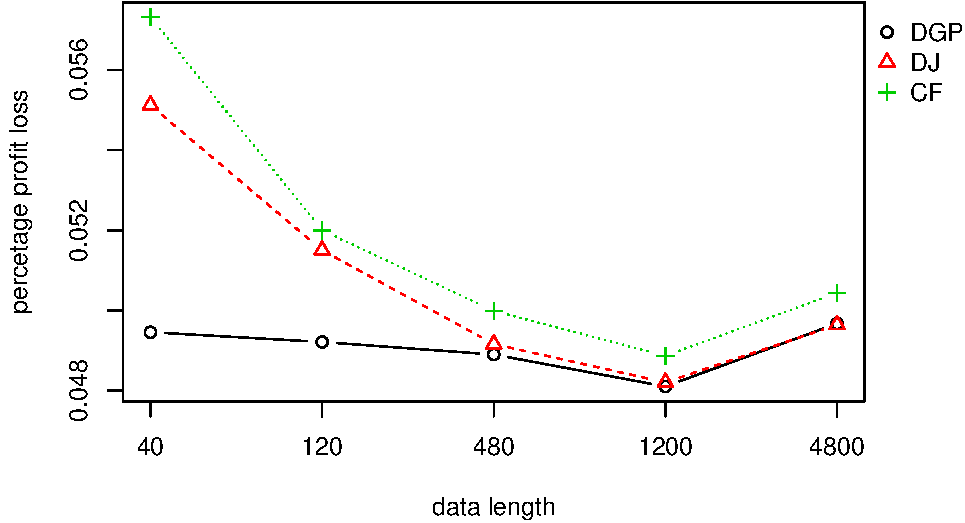
\includegraphics{information-plot_files/figure-latex/SAR(3)(1)_4-1.pdf}

\end{document}
